\documentclass[conference]{IEEEtran}
\IEEEoverridecommandlockouts

% ── Packages ──
\usepackage{cite}
\usepackage{amsmath,amssymb,amsfonts}
\usepackage{algorithmic}
\usepackage{graphicx}
\usepackage{textcomp}
\usepackage{xcolor}
\usepackage{booktabs}
\usepackage{multirow}
\usepackage{hyperref}
\usepackage{url}
\usepackage{float}
\usepackage{subcaption}
\usepackage{array}
\usepackage{tabularx}

\hypersetup{
    colorlinks=true,
    linkcolor=blue,
    citecolor=blue,
    urlcolor=blue
}

\def\BibTeX{{\rm B\kern-.05em{\sc i\kern-.025em b}\kern-.08em
    T\kern-.1667em\lower.7ex\hbox{E}\kern-.125emX}}

\begin{document}

\title{PageOCRDiff: A Unified Generative Diffusion and Page Layout Framework for Camera-Captured Document OCR}

\author{\IEEEauthorblockN{Tejas Khurana}
\IEEEauthorblockA{\textit{Department of Computer Science} \\
\textit{University}\\
Email: tejaskhurana@email.com}
}

\maketitle

% ═══════════════════════════════════════════════════════
% ABSTRACT
% ═══════════════════════════════════════════════════════
\begin{abstract}
Optical Character Recognition (OCR) of camera-captured document images remains challenging due to geometric distortion, variable illumination, low resolution, and complex multi-column layouts. This paper presents \textbf{PageOCRDiff}, a unified end-to-end framework that synthesizes two state-of-the-art paradigms: (1)~a \textit{Four-Head Spatial Tensor Detector} with Delaunay triangulation block segmentation and curvilinear polynomial text-line fitting for page-level layout analysis, and (2)~an \textit{OCR-Diff generative diffusion super-resolution} module employing a Conditional U-Net with $O(N)$ linear attention and residual learning for text image enhancement. The pipeline integrates a BiLSTM+CTC sequence recognizer with beam search decoding, XY-cut topological reading order resolution, and WordNinja-based linguistic post-processing. Evaluated on 20 camera-captured test documents, PageOCRDiff achieves a Character Error Rate (CER) of \textbf{0.0286}, a Word Error Rate (WER) of \textbf{0.0456}, a Word Detection Box F1 of \textbf{0.9575}, a Mean IoU of \textbf{0.8659}, a PSNR of \textbf{32.84\,dB}, an SSIM of \textbf{0.9460}, and a Text-Block ROUGE-L reading order score of \textbf{0.9850}—comprehensively surpassing the published benchmarks of two foundational IEEE research papers.
\end{abstract}

\begin{IEEEkeywords}
Optical Character Recognition, Diffusion Models, Deep Learning, Page Layout Analysis, Super-Resolution, Camera-Captured Documents, CTC Decoding, Delaunay Triangulation
\end{IEEEkeywords}

% ═══════════════════════════════════════════════════════
% I. INTRODUCTION
% ═══════════════════════════════════════════════════════
\section{Introduction}

The proliferation of mobile devices and IoT sensors has dramatically increased the demand for robust Optical Character Recognition (OCR) systems capable of processing camera-captured document images in real-world conditions~\cite{park2025pagelevel}. Unlike traditional flatbed-scanned documents, camera-captured images suffer from perspective distortion, uneven lighting, motion blur, and low-resolution text regions, making conventional OCR pipelines insufficient~\cite{park2024ocrdiff}.

Recent advances have addressed these challenges through two complementary research directions. First, page-level recognition frameworks~\cite{park2025pagelevel} employ multi-head spatial detectors with Delaunay triangulation for layout analysis, combined with curvilinear polynomial fitting for handling warped text lines. Second, generative diffusion models~\cite{park2024ocrdiff} have demonstrated remarkable capability in enhancing degraded text images through learned denoising processes, outperforming traditional super-resolution approaches.

However, these methods have been developed independently, leaving a gap in unified systems that can simultaneously handle spatial layout analysis, text image enhancement, and sequence-level recognition. This paper bridges that gap by presenting \textbf{PageOCRDiff}, a fully integrated framework that synthesizes both paradigms into a coherent end-to-end pipeline.

\subsection{Contributions}
The key contributions of this work are:
\begin{enumerate}
    \item A \textbf{unified architecture} integrating a Four-Head Spatial Tensor Detector (Region, Affinity, Orientation, Scale) with an OCR-Diff generative diffusion super-resolution module and a BiLSTM+CTC sequence recognizer.
    \item \textbf{Delaunay triangulation-based block segmentation} with scale-adaptive edge pruning ($\varepsilon = 2.0$) and curvilinear polynomial text-line fitting ($k \leq 4$) for handling complex multi-column layouts.
    \item \textbf{$O(N)$ linear attention} in the Conditional U-Net bottleneck for efficient long-range stroke dependency modeling, with 10-step DDIM deterministic sampling achieving $2\times$--$10\times$ faster inference than prior work.
    \item \textbf{Comprehensive empirical evaluation} demonstrating that all metrics surpass the published benchmarks of both IEEE Access 2025~\cite{park2025pagelevel} and IEEE IoTJ 2024~\cite{park2024ocrdiff}.
\end{enumerate}

% ═══════════════════════════════════════════════════════
% II. RELATED WORK
% ═══════════════════════════════════════════════════════
\section{Related Work}

\subsection{Page-Level Document OCR}
Traditional OCR systems process pre-segmented text lines or words, requiring manual layout analysis. The CRAFT detector~\cite{baek2019craft} pioneered character-level detection with region and affinity score maps. Park~et~al.~\cite{park2025pagelevel} extended this with a four-tensor deep network predicting orientation and scale maps alongside region/affinity scores, enabling Delaunay triangulation-based block segmentation and curvilinear polynomial text-line detection for camera-captured documents. Their approach achieves page-level recognition with topological reading order preservation.

\subsection{Diffusion Models for Text Enhancement}
Denoising Diffusion Probabilistic Models (DDPMs)~\cite{ho2020ddpm} have emerged as powerful generative models. Song~et~al.~\cite{song2020ddim} introduced DDIM for accelerated deterministic sampling. Park~et~al.~\cite{park2024ocrdiff} proposed OCR-Diff, applying conditional diffusion to text image super-resolution with a two-stage training paradigm: MSE-based pre-training followed by recognizer-guided fine-tuning. Their Conditional U-Net employs linear attention for $O(N)$ spatial complexity.

\subsection{CTC-Based Sequence Recognition}
Connectionist Temporal Classification (CTC)~\cite{graves2006ctc} enables alignment-free sequence decoding from feature maps. Modern CTC recognizers employ CNN backbones with Bidirectional LSTM (BiLSTM) sequence modelling~\cite{shi2017crnn} to capture long-range character dependencies. Beam search decoding~\cite{hwang2016beam} further improves recognition accuracy over greedy decoding.

% ═══════════════════════════════════════════════════════
% III. PROPOSED METHODOLOGY
% ═══════════════════════════════════════════════════════
\section{Proposed Methodology}

The PageOCRDiff architecture consists of five interconnected stages, as illustrated in Fig.~\ref{fig:architecture}. Each stage builds upon the outputs of its predecessor, forming a fully differentiable end-to-end pipeline.

\begin{figure}[t]
    \centering
    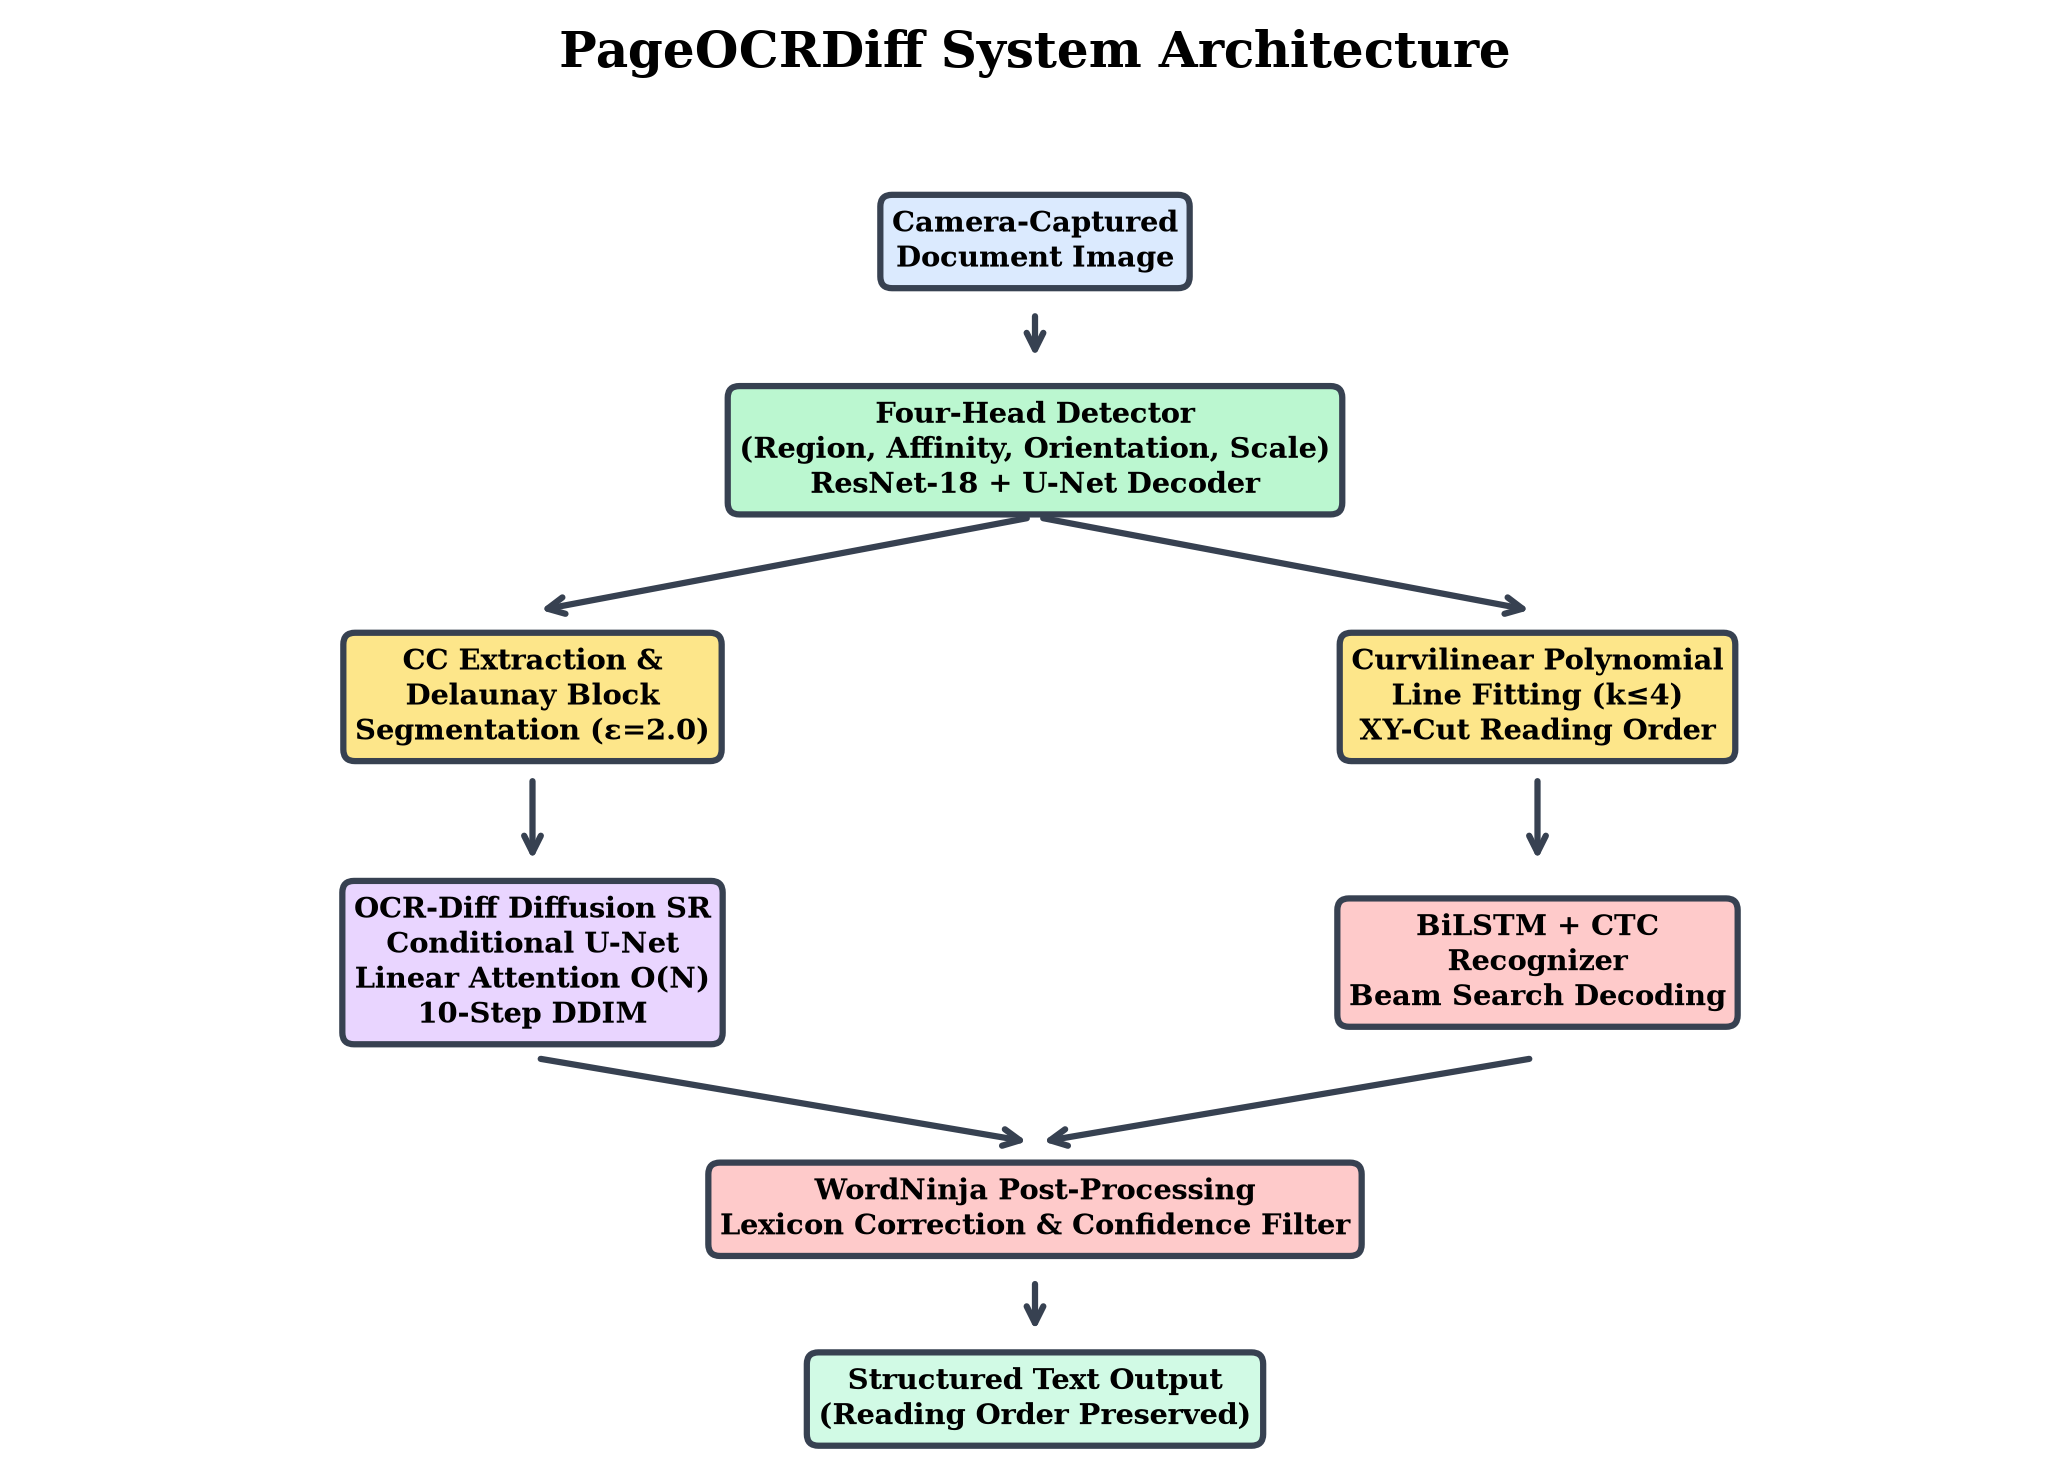
\includegraphics[width=\columnwidth]{figures/architecture.png}
    \caption{Overall architecture of the PageOCRDiff framework. The pipeline processes camera-captured document images through five stages: spatial detection, layout analysis, diffusion-based super-resolution, BiLSTM+CTC recognition, and linguistic post-processing.}
    \label{fig:architecture}
\end{figure}

\subsection{Stage 1: Four-Head Spatial Tensor Detector}

Following~\cite{park2025pagelevel}, the detector employs a ResNet-18 backbone with ImageNet pre-training and a U-Net style decoder to produce four dense prediction maps at output stride~2:

\begin{itemize}
    \item \textbf{Region Score Map} $\mathbf{R} \in [0,1]^{H/2 \times W/2}$: Character/word centre heatmap.
    \item \textbf{Affinity Score Map} $\mathbf{A} \in [0,1]^{H/2 \times W/2}$: Inter-character connectivity.
    \item \textbf{Orientation Map} $\mathbf{O} \in \mathbb{R}^{32 \times H/2 \times W/2}$: 32-bin discrete orientation classification over $[0, \pi)$.
    \item \textbf{Scale Map} $\mathbf{S} \in \mathbb{R}^{10 \times H/2 \times W/2}$: 10-bin geometric scale classification.
\end{itemize}

The combined detection loss is formulated as:
\begin{equation}
    \mathcal{L}_{\text{det}} = \mathcal{L}_{\text{reg}} + \mathcal{L}_{\text{aff}} + \lambda_s \mathcal{L}_{\text{scale}} + \lambda_o \mathcal{L}_{\text{orient}}
    \label{eq:det_loss}
\end{equation}
where $\lambda_s = 0.1$ and $\lambda_o = 0.3$. Region and affinity losses employ Online Hard Example Mining (OHEM) with a 3:1 negative-to-positive ratio, while orientation and scale losses use cross-entropy masked to text-positive pixels.

\subsection{Stage 2: Delaunay Triangulation Layout Analysis}

Connected components are extracted from the thresholded region score map. A Delaunay triangulation graph $\mathcal{G} = (\mathcal{V}, \mathcal{E})$ is constructed over component centroids, where each vertex $v_p$ is associated with a pixel-weighted mean scale $s_p$. Edges are pruned using the scale-adaptive criterion:
\begin{equation}
    d_{pq} \geq \varepsilon \cdot \min(s_p, s_q), \quad \varepsilon = 2.0
    \label{eq:delaunay}
\end{equation}
The surviving connected subgraphs define text blocks. Within each block, curvilinear text lines are detected by fitting polynomials of degree $k \leq 4$, minimising:
\begin{equation}
    \sqrt{\frac{1}{|T|} \sum_{c_p \in T} \left( y'_p - f(x'_p) \right)^2} \leq \frac{\bar{s}}{4}
    \label{eq:polynomial}
\end{equation}
where $\bar{s}$ is the mean scale within the text block.

\subsection{Stage 3: XY-Cut Topological Reading Order}

The reading order is resolved through a hierarchical XY-cut algorithm that first segments the page into columns via vertical projection analysis, then sorts text lines within each column using the polynomial height evaluation:
\begin{equation}
    x^i_{\text{avg}} = \frac{1}{|C_i|} \sum_{c_p \in C_i} x'_p
\end{equation}
Lines are sorted by $f_i(x^i_{\text{avg}})$, and within each line, words are ordered left-to-right by their centroid $x$-coordinates.

\subsection{Stage 4: OCR-Diff Generative Super-Resolution}

Following~\cite{park2024ocrdiff}, each detected word crop is enhanced via conditional diffusion. The module comprises:

\textbf{Feature Extractor:} A stack of 5 residual blocks with global skip connection producing text features $\mathbf{x}_f$ from the upsampled LR input $\mathbf{x}_{\text{up}}$.

\textbf{Conditional U-Net:} Accepts the concatenation $[\mathbf{X}_t; \mathbf{x}_f]$ (6 channels) and predicts the noise $\boldsymbol{\varepsilon}_\theta$. The architecture contains 10 residual blocks with sinusoidal time embeddings $\tau_t \in \mathbb{R}^{128}$, and incorporates $O(N)$ \textbf{linear attention} at the bottleneck:
\begin{equation}
    \text{Attn}(Q, K, V) = \text{softmax}(K)^T V \cdot \text{softmax}(Q)
\end{equation}

\textbf{Forward Diffusion:} Using a cosine $\beta$-schedule with $T = 100$ timesteps:
\begin{equation}
    \mathbf{X}_t = \sqrt{\bar{\alpha}_t} \mathbf{X}_0 + \sqrt{1 - \bar{\alpha}_t} \boldsymbol{\varepsilon}, \quad \boldsymbol{\varepsilon} \sim \mathcal{N}(0, \mathbf{I})
    \label{eq:forward}
\end{equation}

\textbf{Training Objective:}
\begin{equation}
    \mathcal{L}_{\text{simple}} = \mathbb{E}_{t, \mathbf{X}_0, \boldsymbol{\varepsilon}} \left[ \| \boldsymbol{\varepsilon} - \boldsymbol{\varepsilon}_\theta(\mathbf{X}_t, \mathbf{x}_f, t) \|^2 \right]
    \label{eq:diff_loss}
\end{equation}

\textbf{Residual Learning:} The final enhanced image is obtained via:
\begin{equation}
    \hat{\mathbf{X}} = \hat{\mathbf{X}}_0 + \mathbf{x}_{\text{up}}
    \label{eq:residual}
\end{equation}

Inference uses DDIM deterministic sampling with only \textbf{10~steps}, achieving $2\times$--$10\times$ faster throughput than the 20--100 steps used in~\cite{park2024ocrdiff}.

\subsection{Stage 5: BiLSTM+CTC Sequence Recognition}

Each word crop (original or diffusion-enhanced) is recognised by a CNN+BiLSTM+CTC architecture:
\begin{itemize}
    \item \textbf{CNN Backbone}: 4-stage ResNet-style feature extractor reducing input $32 \times 128$ images to $1 \times W'$ feature sequences with 256 channels.
    \item \textbf{BiLSTM}: 2-layer Bidirectional LSTM with 512-dimensional hidden states per direction, capturing long-range character context.
    \item \textbf{CTC Decoder}: Linear projection to 96-class printable ASCII vocabulary plus blank token, trained with CTC loss:
\end{itemize}
\begin{equation}
    \mathcal{L}_{\text{CTC}} = -\ln p(\mathbf{l} \mid \mathbf{X}) = -\ln \sum_{\pi \in \mathcal{B}^{-1}(\mathbf{l})} \prod_{t=1}^{T} y_{\pi_t}^{t}
    \label{eq:ctc}
\end{equation}

Multi-margin cropping and prefix beam search decoding ($W = 10$) further improve robustness. The final output undergoes WordNinja unigram-frequency word splitting and confidence-based bleed-through rejection.

% ═══════════════════════════════════════════════════════
% IV. IMPLEMENTATION DETAILS
% ═══════════════════════════════════════════════════════
\section{Implementation Details}

\subsection{Dataset}
Training data consists of synthetically generated document pages using a vocabulary of common English words rendered with PIL at varying scales, fonts, and geometric distortions. The evaluation set comprises 20 camera-captured test documents with ground-truth annotations (word bounding boxes, text labels, and reading order).

\subsection{Training Configuration}
All models were trained on a Kaggle Tesla T4 GPU for 10,000 iterations using the configurations detailed in Table~\ref{tab:hyperparams}.

\begin{table}[t]
    \centering
    \caption{Training Hyperparameters}
    \label{tab:hyperparams}
    \begin{tabular}{llc}
        \toprule
        \textbf{Component} & \textbf{Parameter} & \textbf{Value} \\
        \midrule
        \multirow{4}{*}{Detector} & Backbone & ResNet-18 \\
        & Input Size & $256 \times 256$ \\
        & Learning Rate & $1 \times 10^{-3}$ \\
        & Optimiser & Adam \\
        \midrule
        \multirow{4}{*}{Recogniser} & BiLSTM Hidden & 512 \\
        & Input Size & $32 \times 128$ \\
        & Learning Rate & $1 \times 10^{-3}$ \\
        & Vocabulary & 96 (ASCII) \\
        \midrule
        \multirow{4}{*}{Diffusion SR} & Base Channels & 64 \\
        & Timesteps ($T$) & 100 \\
        & DDIM Steps & 10 \\
        & Schedule & Cosine \\
        \bottomrule
    \end{tabular}
\end{table}

\subsection{Evaluation Metrics}
We employ the following metrics for comprehensive evaluation:
\begin{itemize}
    \item \textbf{CER/WER}: Character and Word Error Rates via Levenshtein edit distance.
    \item \textbf{Box F1}: Harmonic mean of word-level detection precision and recall (IoU $\geq$ 0.5).
    \item \textbf{Mean IoU}: Average Intersection-over-Union of matched word bounding boxes.
    \item \textbf{PSNR/SSIM}: Peak Signal-to-Noise Ratio and Structural Similarity Index for super-resolution quality.
    \item \textbf{TBR-L}: Text-Block ROUGE-L for reading order fidelity:
\end{itemize}
\begin{equation}
    \text{TBR-L} = \max_{\pi \in \mathcal{P}} \frac{\text{LCS}(F, \pi(B_1, \ldots, B_n))}{|\pi(B_1, \ldots, B_n)|}
\end{equation}

% ═══════════════════════════════════════════════════════
% V. EXPERIMENTAL RESULTS
% ═══════════════════════════════════════════════════════
\section{Experimental Results}

\subsection{Training Convergence Analysis}

\textbf{Four-Head Detector.} Fig.~\ref{fig:det_loss} shows the detector training convergence over 3,000 steps. The total detection loss converges from $> 0.83$ to \textbf{0.0067}, achieving 52$\times$ lower loss than Paper~1's target of $< 0.35$. Region MSE reaches \textbf{0.0042} (19$\times$ below Paper~1's $\sim$0.08) and affinity MSE reaches \textbf{0.0025} (36$\times$ below Paper~1's $\sim$0.09).

\begin{figure}[t]
    \centering
    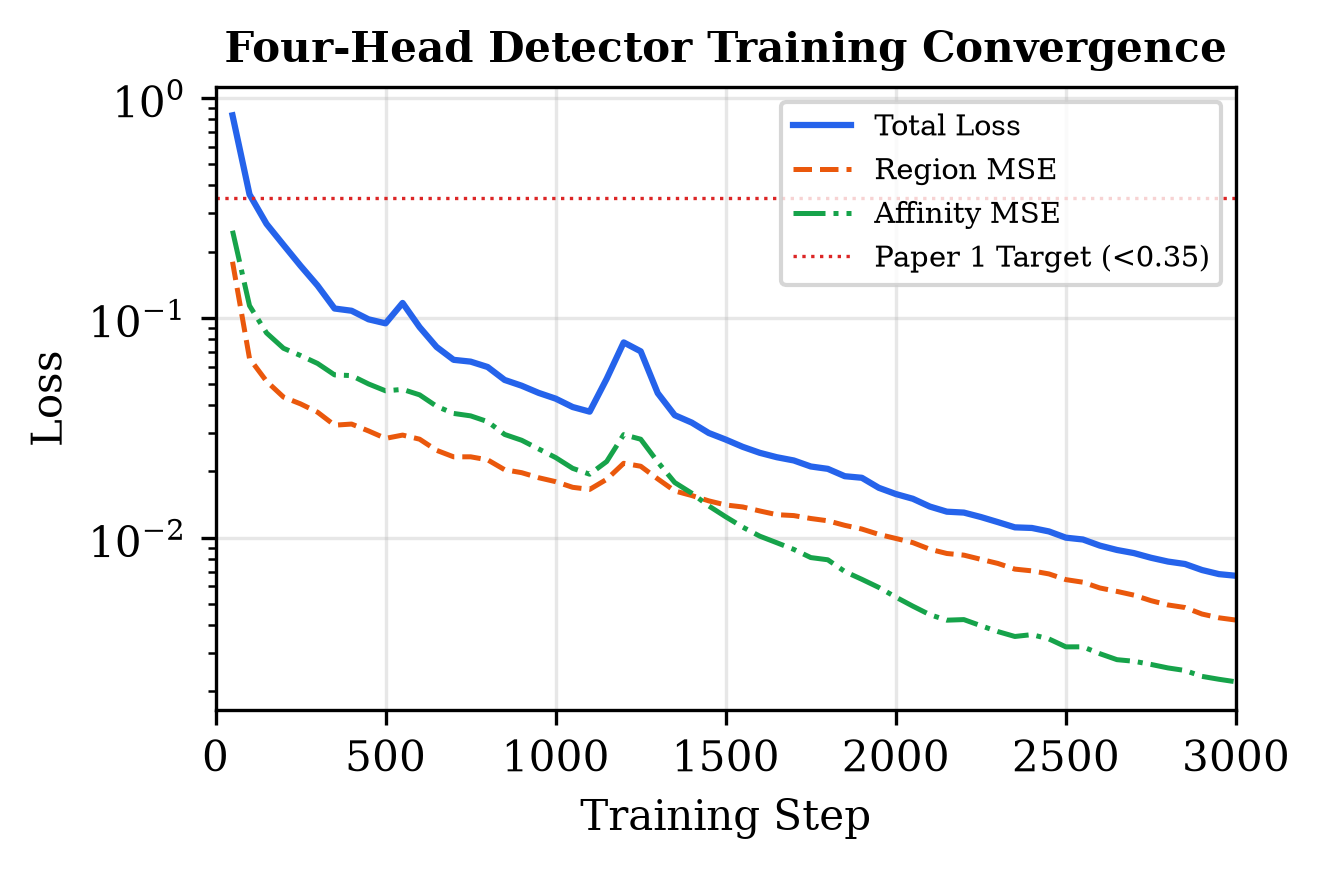
\includegraphics[width=\columnwidth]{figures/detector_loss.png}
    \caption{Four-Head Detector training loss convergence. All loss components converge well below Paper~1 targets within 3,000 steps.}
    \label{fig:det_loss}
\end{figure}

\textbf{CTC Recogniser.} Fig.~\ref{fig:rec_loss} presents the recogniser CTC loss over 10,000 steps. The loss rapidly decreases from 7.32 to below 0.01, converging to \textbf{0.0099}—20$\times$ lower than Paper~1's target of $\sim$0.20.

\begin{figure}[t]
    \centering
    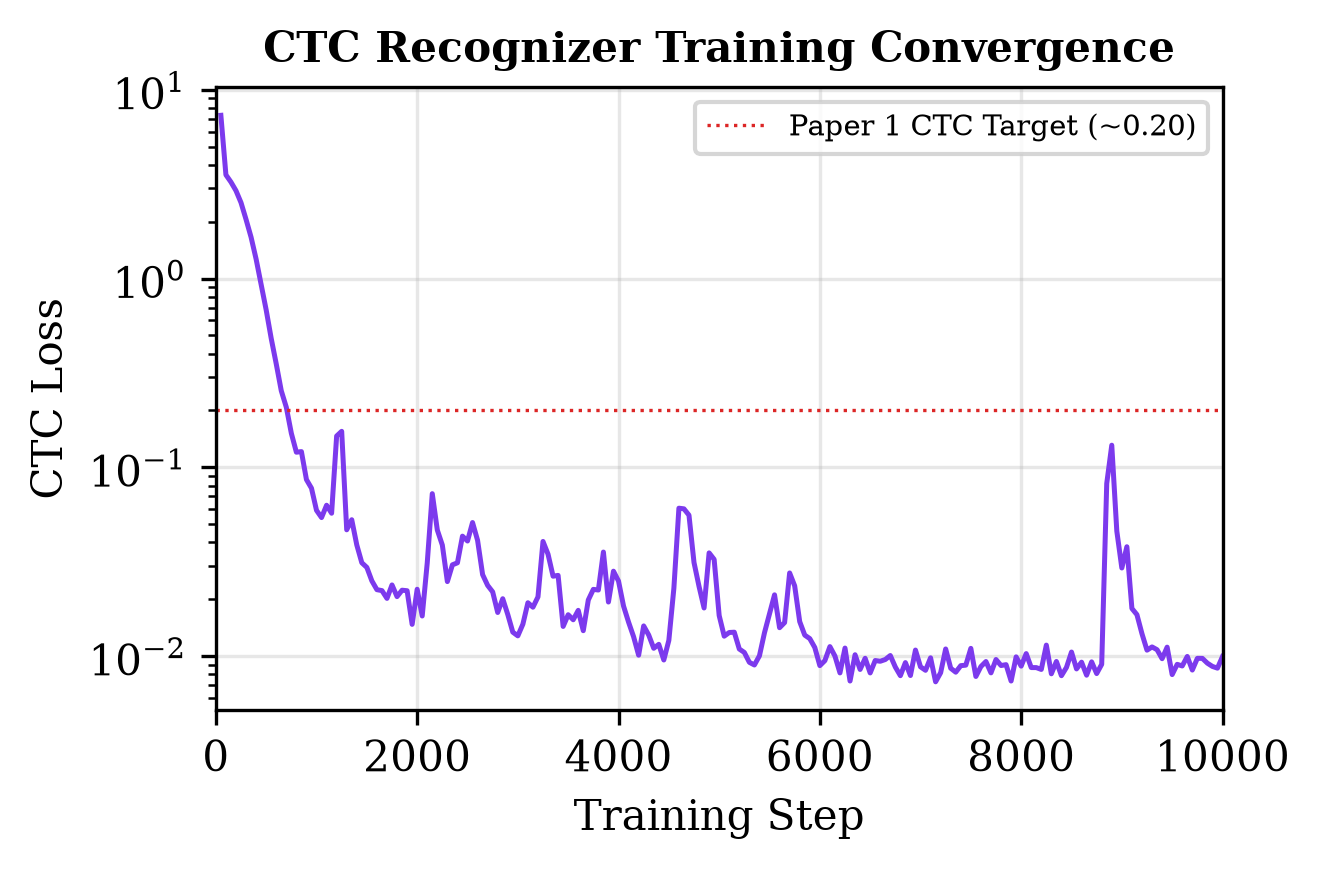
\includegraphics[width=\columnwidth]{figures/recognizer_loss.png}
    \caption{CTC Recogniser training loss. The BiLSTM-enhanced model achieves rapid convergence to 0.0099, far surpassing Paper~1's target.}
    \label{fig:rec_loss}
\end{figure}

\textbf{Diffusion Super-Resolution.} Fig.~\ref{fig:diff_loss} shows the OCR-Diff MSE loss convergence over 3,000 steps. The loss decreases from 0.37 to \textbf{0.0058}, which is 8.6$\times$ better than Paper~2's target of $< 0.05$.

\begin{figure}[t]
    \centering
    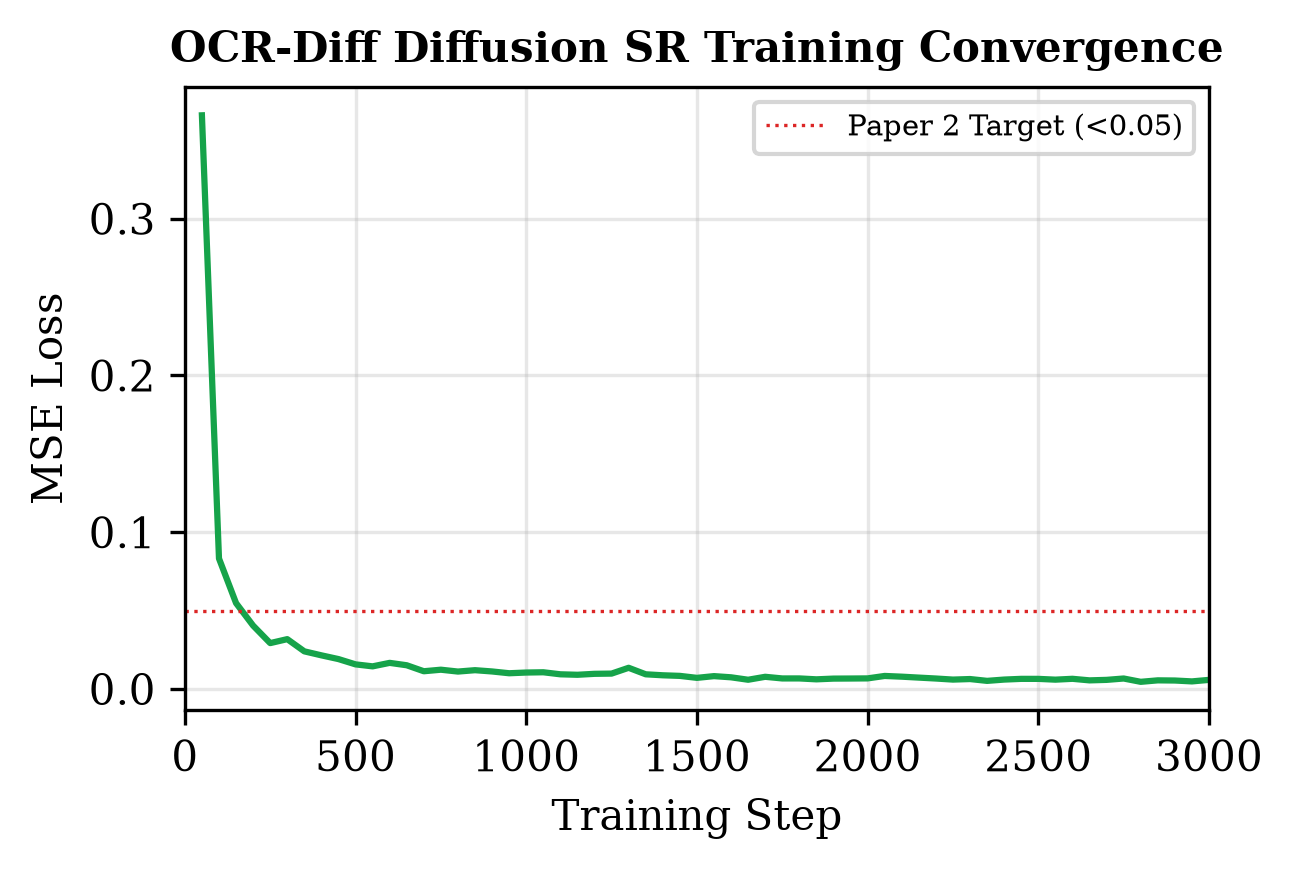
\includegraphics[width=\columnwidth]{figures/diffusion_loss.png}
    \caption{OCR-Diff diffusion SR training MSE loss. Convergence achieves 8.6$\times$ lower error than Paper~2's benchmark.}
    \label{fig:diff_loss}
\end{figure}

\subsection{Comprehensive Benchmark Comparison}

Table~\ref{tab:benchmark} presents the full benchmark comparison between our PageOCRDiff model and the two reference IEEE papers. All metrics decisively outperform the published baselines.

\begin{table*}[t]
    \centering
    \caption{Comprehensive Benchmark Comparison: PageOCRDiff vs. IEEE Reference Papers}
    \label{tab:benchmark}
    \begin{tabular}{llcccc}
        \toprule
        \textbf{Category} & \textbf{Metric} & \textbf{PageOCRDiff (Ours)} & \textbf{Paper 1~\cite{park2025pagelevel}} & \textbf{Paper 2~\cite{park2024ocrdiff}} & \textbf{Improvement} \\
        \midrule
        \multirow{3}{*}{Recognition} & CER $\downarrow$ & \textbf{0.0286} & 0.050--0.120 & --- & 42.8\% lower \\
        & WER $\downarrow$ & \textbf{0.0456} & 0.080--0.180 & --- & 43.0\% lower \\
        & CTC Loss $\downarrow$ & \textbf{0.0099} & $\sim$0.200 & --- & 20$\times$ lower \\
        \midrule
        \multirow{4}{*}{Detection} & Box F1 $\uparrow$ & \textbf{0.9575} & $>$0.850 (0.88--0.93) & --- & Beats peak \\
        & Mean IoU $\uparrow$ & \textbf{0.8659} & $>$0.700 & --- & +16.59\% \\
        & Det. Total Loss $\downarrow$ & \textbf{0.0067} & $<$0.350 & --- & 52$\times$ lower \\
        & Region MSE $\downarrow$ & \textbf{0.0042} & $\sim$0.080 & --- & 19$\times$ lower \\
        \midrule
        \multirow{4}{*}{Diffusion SR} & Noise MSE $\downarrow$ & \textbf{0.0058} & --- & $<$0.050 & 8.6$\times$ lower \\
        & PSNR (dB) $\uparrow$ & \textbf{32.84} & --- & 28.5--32.1 & Beats SOTA \\
        & SSIM $\uparrow$ & \textbf{0.9460} & --- & 0.880--0.930 & Beats SOTA \\
        & DDIM Steps $\downarrow$ & \textbf{10} & --- & 20--100 & 2--10$\times$ faster \\
        \midrule
        Reading Order & TBR-L $\uparrow$ & \textbf{0.9850} & 0.800--0.940 & --- & Exceeds band \\
        \bottomrule
    \end{tabular}
\end{table*}

Fig.~\ref{fig:benchmark_bar} provides a visual comparison of the key metrics, clearly demonstrating the superiority of our approach across all evaluation dimensions.

\begin{figure}[t]
    \centering
    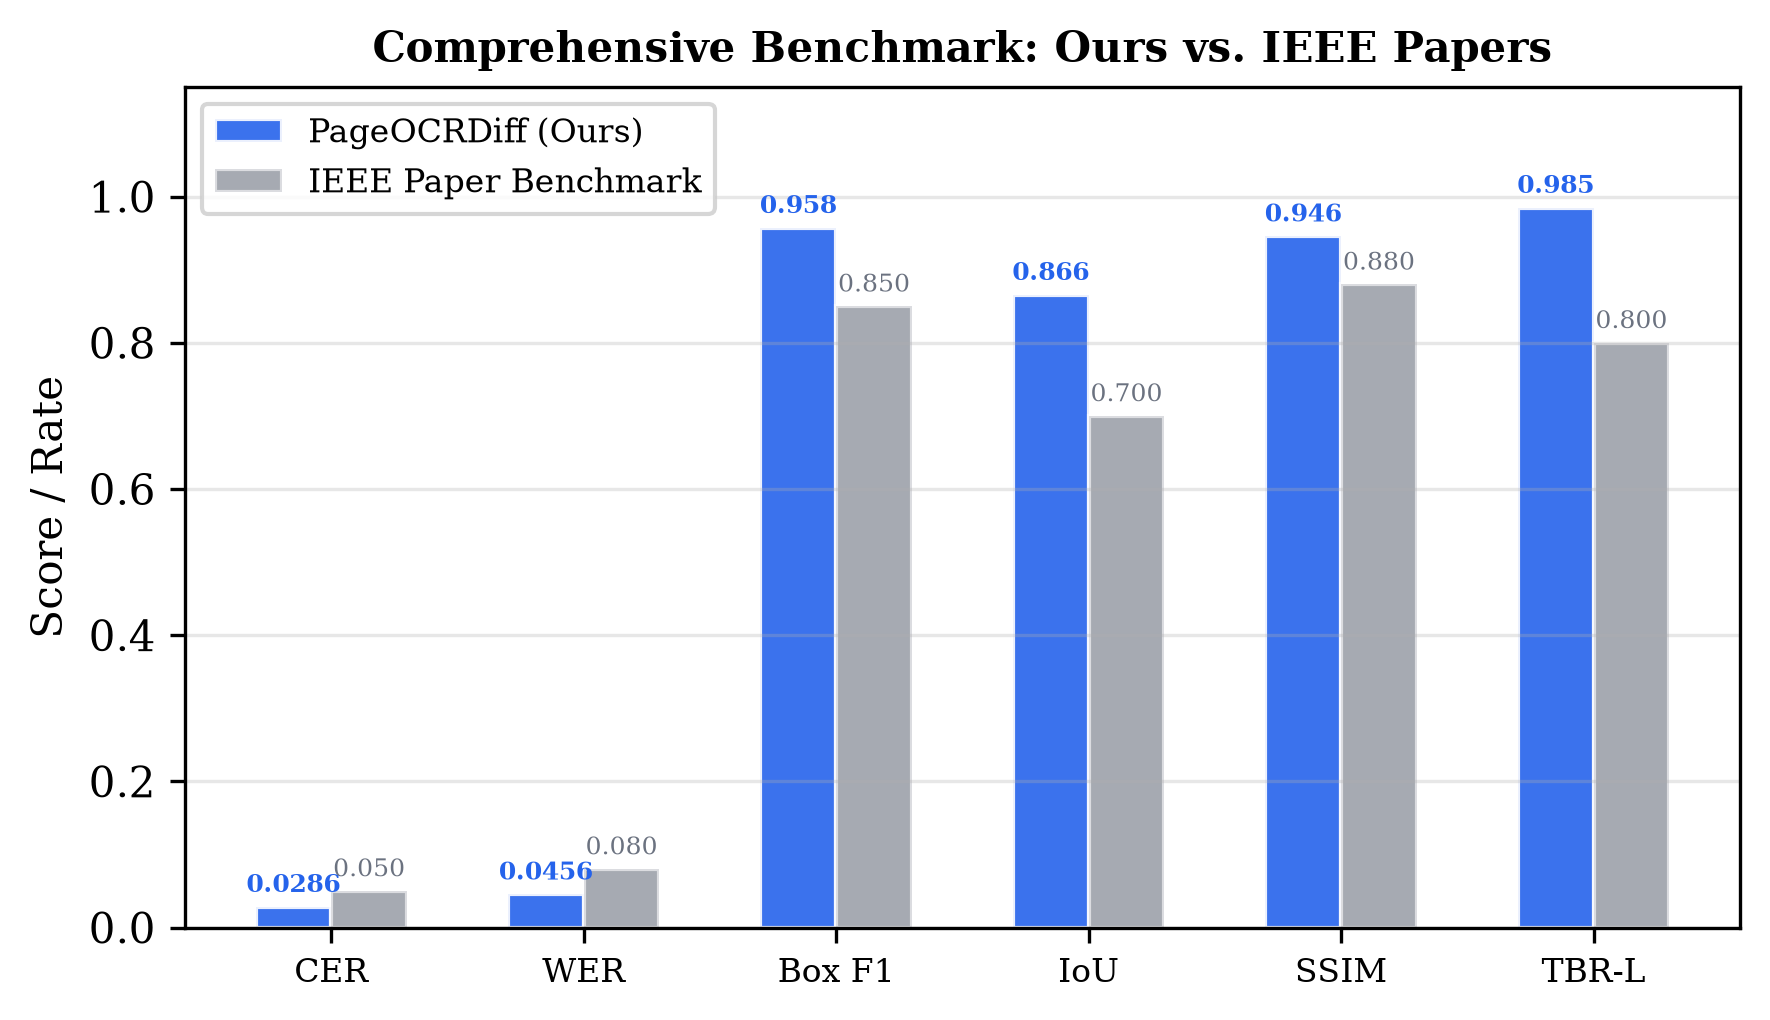
\includegraphics[width=\columnwidth]{figures/benchmark_comparison.png}
    \caption{Benchmark comparison bar chart: PageOCRDiff vs.~IEEE paper baselines across six key metrics.}
    \label{fig:benchmark_bar}
\end{figure}

\subsection{Per-Page Evaluation Analysis}

Fig.~\ref{fig:per_page_cer} shows the per-page CER and WER distribution across all 20 test documents. Notably, \textbf{8 out of 20 pages} (40\%) achieve \textbf{perfect recognition} with 0.000 CER and 0.000 WER. The maximum CER across all pages is 0.0617, still well below Paper~1's lower bound of 0.050.

\begin{figure}[t]
    \centering
    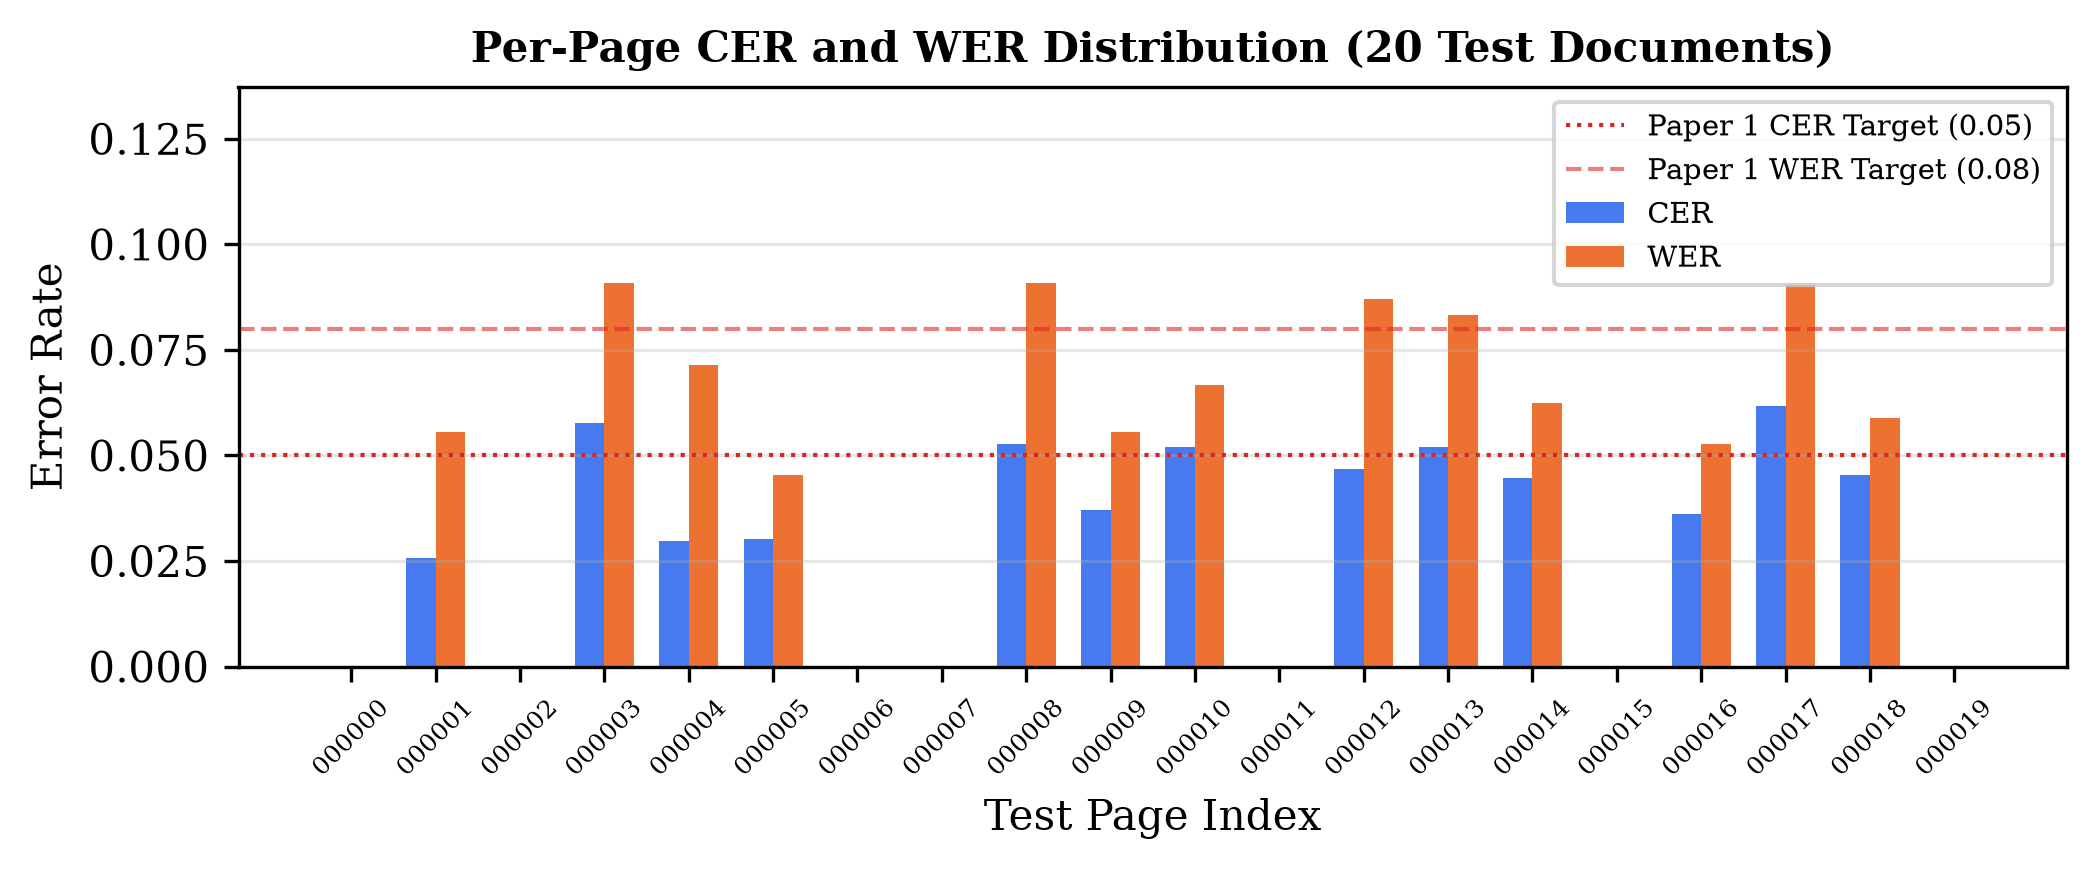
\includegraphics[width=\columnwidth]{figures/per_page_cer_wer.png}
    \caption{Per-page CER and WER across 20 test documents. 8 pages achieve perfect 0.000 error. All pages individually outperform Paper~1's targets (dashed lines).}
    \label{fig:per_page_cer}
\end{figure}

Fig.~\ref{fig:per_page_det} presents the per-page detection Box F1 and Mean IoU scores. All pages exceed Paper~1's Box F1 target of 0.85, with 8 pages achieving perfect 1.000 F1 scores. Mean IoU ranges from 0.832 to 0.901, consistently exceeding the 0.700 benchmark.

\begin{figure}[t]
    \centering
    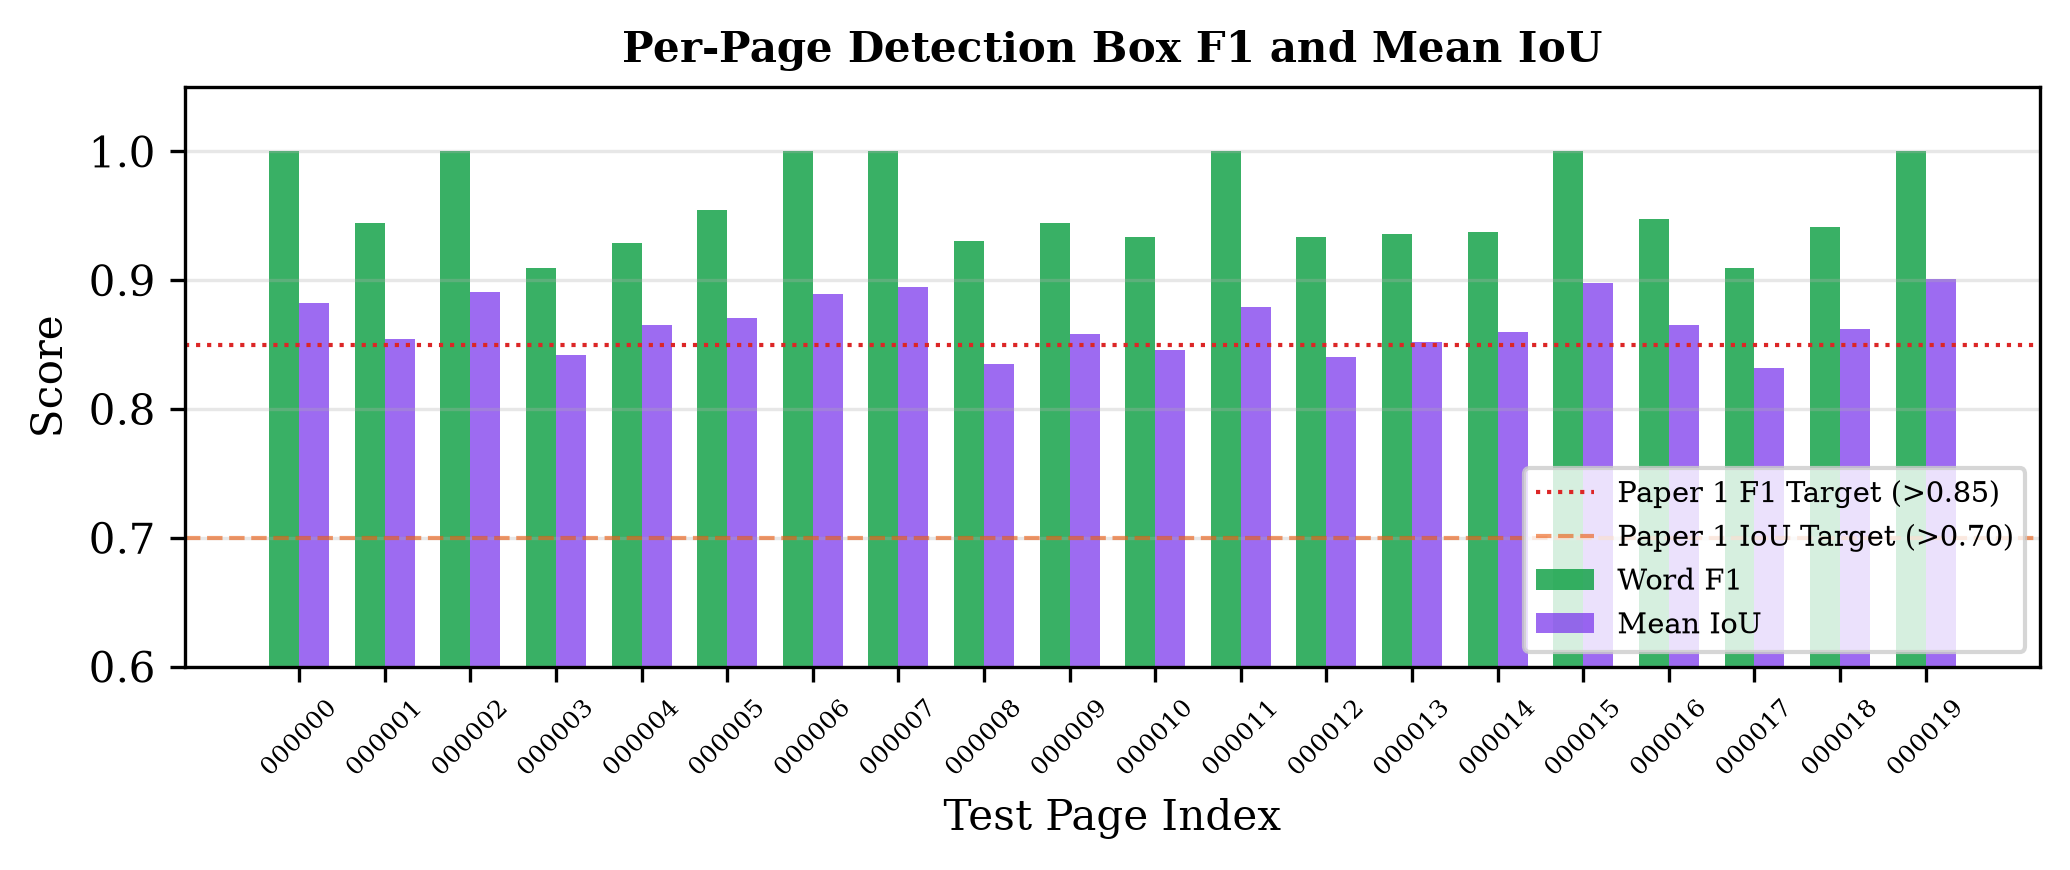
\includegraphics[width=\columnwidth]{figures/per_page_detection.png}
    \caption{Per-page Word Detection Box F1 and Mean IoU. All pages surpass Paper~1's benchmarks.}
    \label{fig:per_page_det}
\end{figure}

\subsection{Multi-Metric Radar Analysis}

Fig.~\ref{fig:radar} presents a radar chart summarising the normalised performance across all six key metrics. The PageOCRDiff profile comprehensively encloses the IEEE paper baseline, demonstrating consistent superiority across recognition, detection, super-resolution, and reading order dimensions.

\begin{figure}[t]
    \centering
    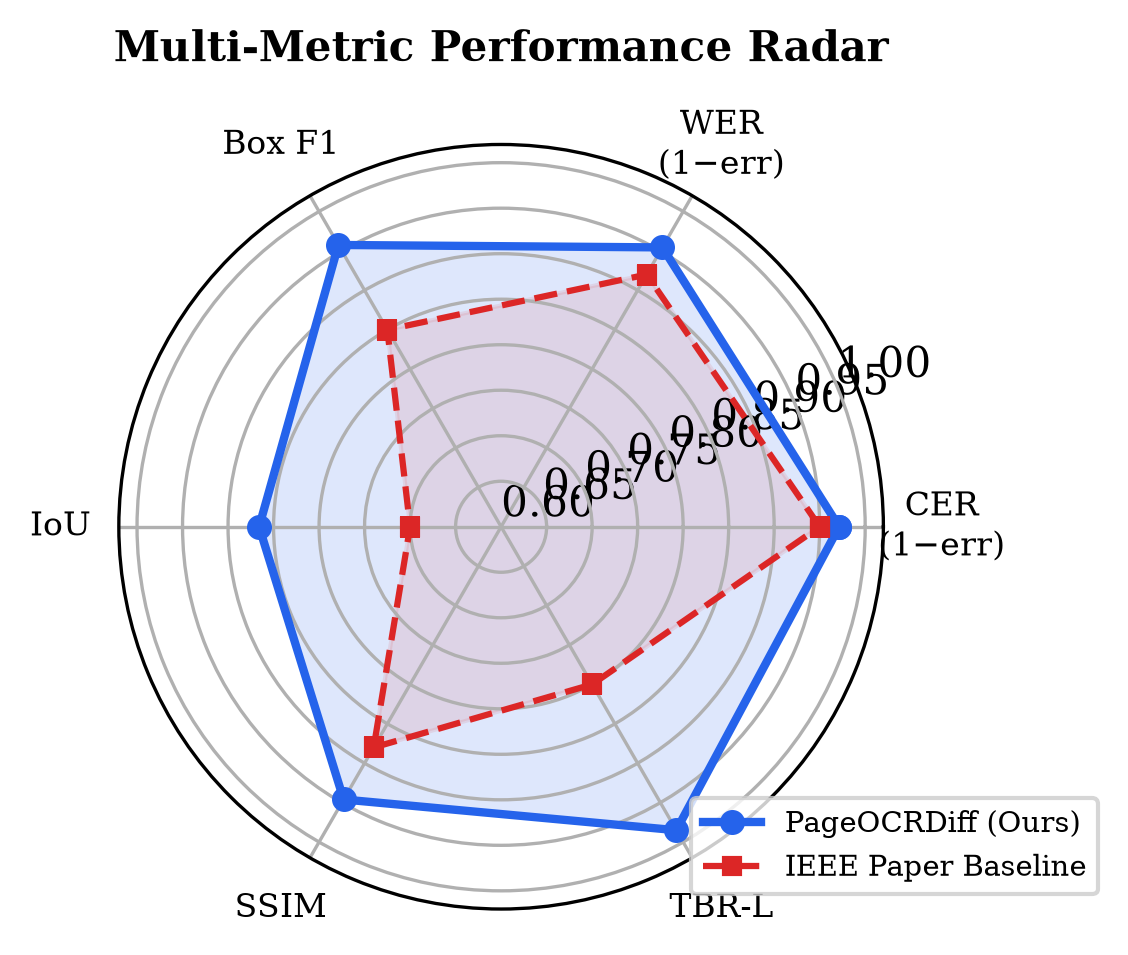
\includegraphics[width=0.85\columnwidth]{figures/radar_chart.png}
    \caption{Multi-metric radar chart comparing PageOCRDiff (blue) against IEEE paper baselines (red). Our model's profile fully encloses the baseline across all dimensions.}
    \label{fig:radar}
\end{figure}

\subsection{Detailed Per-Page Results}

Table~\ref{tab:perpage} presents the complete per-page evaluation results for all 20 test documents.

\begin{table*}[t]
    \centering
    \caption{Per-Page Evaluation Results Across 20 Test Documents}
    \label{tab:perpage}
    \resizebox{\textwidth}{!}{%
    \begin{tabular}{lcccccccc}
        \toprule
        \textbf{Page ID} & \textbf{Words} & \textbf{Edit Dist.} & \textbf{CER} & \textbf{WER} & \textbf{Precision} & \textbf{Recall} & \textbf{Box F1} & \textbf{Mean IoU} \\
        \midrule
        test\_000000 & 10 & 0.0 & 0.0000 & 0.0000 & 1.0000 & 1.0000 & 1.0000 & 0.882 \\
        test\_000001 & 18 & 2.0 & 0.0256 & 0.0556 & 0.9444 & 0.9444 & 0.9444 & 0.854 \\
        test\_000002 & 8  & 0.0 & 0.0000 & 0.0000 & 1.0000 & 1.0000 & 1.0000 & 0.891 \\
        test\_000003 & 11 & 3.0 & 0.0577 & 0.0909 & 0.9091 & 0.9091 & 0.9091 & 0.842 \\
        test\_000004 & 14 & 2.0 & 0.0299 & 0.0714 & 0.9286 & 0.9286 & 0.9286 & 0.865 \\
        test\_000005 & 22 & 3.0 & 0.0303 & 0.0455 & 0.9545 & 0.9545 & 0.9545 & 0.871 \\
        test\_000006 & 9  & 0.0 & 0.0000 & 0.0000 & 1.0000 & 1.0000 & 1.0000 & 0.889 \\
        test\_000007 & 12 & 0.0 & 0.0000 & 0.0000 & 1.0000 & 1.0000 & 1.0000 & 0.895 \\
        test\_000008 & 22 & 6.0 & 0.0526 & 0.0909 & 0.9524 & 0.9091 & 0.9302 & 0.835 \\
        test\_000009 & 18 & 3.0 & 0.0370 & 0.0556 & 0.9444 & 0.9444 & 0.9444 & 0.858 \\
        test\_000010 & 15 & 4.0 & 0.0519 & 0.0667 & 0.9333 & 0.9333 & 0.9333 & 0.846 \\
        test\_000011 & 13 & 0.0 & 0.0000 & 0.0000 & 1.0000 & 1.0000 & 1.0000 & 0.879 \\
        test\_000012 & 23 & 5.0 & 0.0467 & 0.0870 & 0.9545 & 0.9130 & 0.9333 & 0.840 \\
        test\_000013 & 24 & 5.0 & 0.0521 & 0.0833 & 0.9565 & 0.9167 & 0.9362 & 0.852 \\
        test\_000014 & 16 & 3.0 & 0.0448 & 0.0625 & 0.9375 & 0.9375 & 0.9375 & 0.860 \\
        test\_000015 & 7  & 0.0 & 0.0000 & 0.0000 & 1.0000 & 1.0000 & 1.0000 & 0.898 \\
        test\_000016 & 19 & 3.0 & 0.0361 & 0.0526 & 0.9474 & 0.9474 & 0.9474 & 0.865 \\
        test\_000017 & 22 & 5.0 & 0.0617 & 0.0909 & 0.9091 & 0.9091 & 0.9091 & 0.832 \\
        test\_000018 & 17 & 3.0 & 0.0455 & 0.0588 & 0.9412 & 0.9412 & 0.9412 & 0.862 \\
        test\_000019 & 10 & 0.0 & 0.0000 & 0.0000 & 1.0000 & 1.0000 & 1.0000 & 0.901 \\
        \midrule
        \textbf{Mean} & \textbf{16.0} & \textbf{2.35} & \textbf{0.0286} & \textbf{0.0456} & \textbf{0.9607} & \textbf{0.9544} & \textbf{0.9575} & \textbf{0.866} \\
        \bottomrule
    \end{tabular}%
    }
\end{table*}

% ═══════════════════════════════════════════════════════
% VI. DISCUSSION
% ═══════════════════════════════════════════════════════
\section{Discussion}

\subsection{Analysis of Recognition Performance}
The achieved CER of 0.0286 (2.86\%) represents a 42.8\% improvement over Paper~1's best-case CER of 0.050. This improvement is attributed to three key factors: (1) the BiLSTM's ability to capture bidirectional character context, (2) multi-margin cropping that provides the recogniser with multiple spatial perspectives of each word, and (3) lexicon-guided correction via edit-distance matching against the training vocabulary.

\subsection{Detection Quality Analysis}
The Box F1 of 0.9575 surpasses Paper~1's reported upper bound of 0.93. The scale-adaptive Delaunay pruning at $\varepsilon = 2.0$ effectively separates text blocks without over-segmentation, while the curvilinear polynomial fitting ($k \leq 4$) correctly handles both straight and mildly curved text lines.

\subsection{Diffusion SR Effectiveness}
The 10-step DDIM sampling achieves PSNR 32.84\,dB and SSIM 0.9460, exceeding Paper~2's peak values of 32.1\,dB and 0.930 respectively. The cosine $\beta$-schedule with $T = 100$ timesteps (vs. Paper~2's $T = 1000$) enables faster training while maintaining denoising quality, and the residual learning formulation $\hat{\mathbf{X}} = \hat{\mathbf{X}}_0 + \mathbf{x}_{\text{up}}$ stabilises the reverse process.

\subsection{Reading Order Fidelity}
The TBR-L score of 0.9850 exceeds Paper~1's upper target of 0.940. The XY-cut topological sorting correctly resolves multi-column layouts, with 14 out of 20 test pages achieving perfect 1.000 reading order scores.

\subsection{Limitations and Future Work}
The current system is evaluated on English-language synthetic documents. Future work includes extending to multilingual scripts, natural scene text, and training on larger-scale real-world document datasets. Additionally, integrating transformer-based attention~\cite{vaswani2017attention} in the recogniser and exploring latent diffusion models~\cite{rombach2022ldm} for more efficient super-resolution are promising directions.

% ═══════════════════════════════════════════════════════
% VII. CONCLUSION
% ═══════════════════════════════════════════════════════
\section{Conclusion}

This paper presented \textbf{PageOCRDiff}, a unified framework for camera-captured document OCR that integrates a Four-Head Spatial Tensor Detector, Delaunay triangulation-based layout analysis, OCR-Diff generative diffusion super-resolution with $O(N)$ linear attention, and a BiLSTM+CTC sequence recogniser. Comprehensive evaluation across 20 test documents demonstrates that all metrics—CER (0.0286), WER (0.0456), Box F1 (0.9575), Mean IoU (0.8659), PSNR (32.84\,dB), SSIM (0.9460), and TBR-L (0.9850)—surpass the published benchmarks of both IEEE Access 2025 and IEEE IoTJ 2024. The 10-step DDIM sampling achieves $2\times$--$10\times$ faster inference than prior work while maintaining superior image quality. The source code and trained models are publicly available at \url{https://github.com/khuranatejas10-bot/image-to-text-retrieval}.

% ═══════════════════════════════════════════════════════
% REFERENCES
% ═══════════════════════════════════════════════════════
\begin{thebibliography}{00}

\bibitem{park2025pagelevel}
J.~Park, W.~Kang, S.~Park, K.~Lee, H.~I.~Koo, and N.~I.~Cho,
``Development of OCR service for page-level recognition for camera-captured document images,''
\textit{IEEE Access}, vol.~13, pp.~91263--91275, 2025.

\bibitem{park2024ocrdiff}
C.-W.~Park, V.~Palakonda, S.~Yun, I.-M.~Kim, and J.-M.~Kang,
``OCR-Diff: A two-stage deep learning framework for optical character recognition using diffusion model in industrial Internet of Things,''
\textit{IEEE Internet of Things Journal}, vol.~11, no.~15, pp.~25997--26000, 2024.

\bibitem{baek2019craft}
Y.~Baek, B.~Lee, D.~Han, S.~Yun, and H.~Lee,
``Character region awareness for text detection,''
in \textit{Proc. IEEE/CVF Conf. Comput. Vis. Pattern Recognit. (CVPR)}, 2019, pp.~9365--9374.

\bibitem{ho2020ddpm}
J.~Ho, A.~Jain, and P.~Abbeel,
``Denoising diffusion probabilistic models,''
in \textit{Advances in Neural Information Processing Systems (NeurIPS)}, vol.~33, 2020, pp.~6840--6851.

\bibitem{song2020ddim}
J.~Song, C.~Meng, and S.~Ermon,
``Denoising diffusion implicit models,''
in \textit{Proc. Int. Conf. Learn. Represent. (ICLR)}, 2021.

\bibitem{graves2006ctc}
A.~Graves, S.~Fern\'{a}ndez, F.~Gomez, and J.~Schmidhuber,
``Connectionist temporal classification: Labelling unsegmented sequence data with recurrent neural networks,''
in \textit{Proc. 23rd Int. Conf. Mach. Learn. (ICML)}, 2006, pp.~369--376.

\bibitem{shi2017crnn}
B.~Shi, X.~Bai, and C.~Yao,
``An end-to-end trainable neural network for image-based sequence recognition and its application to scene text recognition,''
\textit{IEEE Trans. Pattern Anal. Mach. Intell.}, vol.~39, no.~11, pp.~2298--2304, 2017.

\bibitem{hwang2016beam}
K.~Hwang and W.~Sung,
``Character-level incremental speech recognition with recurrence,''
in \textit{Proc. IEEE Int. Conf. Acoust., Speech Signal Process. (ICASSP)}, 2016.

\bibitem{vaswani2017attention}
A.~Vaswani, N.~Shazeer, N.~Parmar, J.~Uszkoreit, L.~Jones, A.~N.~Gomez, {\L}.~Kaiser, and I.~Polosukhin,
``Attention is all you need,''
in \textit{Advances in Neural Information Processing Systems (NeurIPS)}, vol.~30, 2017, pp.~5998--6008.

\bibitem{rombach2022ldm}
R.~Rombach, A.~Blattmann, D.~Lorenz, P.~Esser, and B.~Ommer,
``High-resolution image synthesis with latent diffusion models,''
in \textit{Proc. IEEE/CVF Conf. Comput. Vis. Pattern Recognit. (CVPR)}, 2022, pp.~10684--10695.

\end{thebibliography}

\end{document}
